%\documentclass[a4paper]{article}
\usepackage[utf8]{inputenc}
\usepackage[spanish, es-tabla, es-noshorthands]{babel}
\usepackage[table,xcdraw]{xcolor}
\usepackage[a4paper, footnotesep=1.25cm, headheight=1.25cm, top=2.54cm, left=2.54cm, bottom=2.54cm, right=2.54cm]{geometry}
%\geometry{showframe}

%\usepackage{wrapfig}			%Wrap figure in text
\usepackage[export]{adjustbox}	%Move images
\usepackage{changepage}			%Move tables

\usepackage{tikz}
\usepackage{amsmath}
\usepackage{amsfonts}
\usepackage{amssymb}
\usepackage{float}
\usepackage{graphicx}
\usepackage{caption}
\usepackage{subcaption}
\usepackage{multicol}
\usepackage{multirow}
\usepackage{wrapfig}
\setlength{\doublerulesep}{\arrayrulewidth}
\usepackage{booktabs}
\usepackage[numbib, nottoc, notlot, notlof]{tocbibind}

\usepackage{hyperref}
\hypersetup{
    colorlinks=true,
    linkcolor=blue,
    filecolor=magenta,      
    urlcolor=blue,
    citecolor=blue,    
}

%Change Font Size

% #1 = size, #2 = text
\newcommand{\setparagraphsize}[2]{{\fontsize{#1}{6}\selectfont#2 \par}}		%Cambia el size de todo el parrafo
\newcommand{\setlinesize}[2]{{\fontsize{#1}{6}\selectfont#2}}				%Cambia el font de una oración

\newcommand{\note}[1]{
	\begin{center}
		\huge{ \textcolor{red}{#1} }
	\end{center}
}

%FONTS (IMPORTANTE): Compilar en XeLaTex o LuaLaTeX
\usepackage{anyfontsize}	%Font size
\usepackage{fontspec}		%Font type

\usepackage{etoolbox}
\usepackage{todonotes}

\newcommand{\observacion}[2]{  \ifnumequal{1}{#1}{ { \todo[inline,backgroundcolor=red!25,bordercolor=red!100]{\textbf{Observación: #2}} } }{  }  }

\setcounter{topnumber}{2}
\setcounter{bottomnumber}{2}
\setcounter{totalnumber}{4}
\renewcommand{\topfraction}{0.85}
\renewcommand{\bottomfraction}{0.85}
\renewcommand{\textfraction}{0.15}
\renewcommand{\floatpagefraction}{0.8}
\renewcommand{\textfraction}{0.1}
\setlength{\floatsep}{5pt plus 2pt minus 2pt}
\setlength{\textfloatsep}{5pt plus 2pt minus 2pt}
\setlength{\intextsep}{5pt plus 2pt minus 2pt}

\newcommand{\quotes}[1]{``#1''}
\usepackage{array}
\newcolumntype{C}[1]{>{\centering\let\newline\\\arraybackslash\hspace{0pt}}m{#1}}
\usepackage[american]{circuitikz}
\usetikzlibrary{calc}
\usepackage{fancyhdr}
\usepackage{units} 

\graphicspath{{../Control de posición no lineal/}{../Control de fuerza no lineal/}{../Control híbrido no lineal/}{../Referencias/}{../Deducción de modelo/}{../Conclusiones/}}

\pagestyle{fancy}
\fancyhf{}
\lhead{22.99 - Automación Industrial}
\rhead{Lambertucci, Londero B., Maselli, Mechoulam}
\rfoot{Página \thepage}

%Items con bullets y no cuadrados
\renewcommand{\labelitemi}{\textbullet }

%
%\begin{document}
\Subsection{Caracterización de la señales de entrada y perturbación}
La señal de entrada será un escalón, la cual será la referencia a seguir, y esta apenas entra al sistema atravesará un filtro pasa bajos, para que el cambio de referencia resulte gradual para el sistema.
Adicionalmente en el segundo 10 se perturba al péndulo al aplicarle una fuerza sobre el segundo link. Y luego en el segundo 18 de simulación se procede a desactivar el sistema de control, por lo que se perderá la condición de equilibrio.
\Subsection{Realimentación de Estados}

En la Figura (\ref{fig:realim_posref}) y a lo largo de todas las demás figuras se puede observar la típica respuesta a un sistema con singularidades en el semiplano derecho. Esta respuesa se ve caracterizada por un pequeño desplazamiento hacia la dirección contraria respecto de la señal de referencia.

\begin{figure}[H]
	\centering
	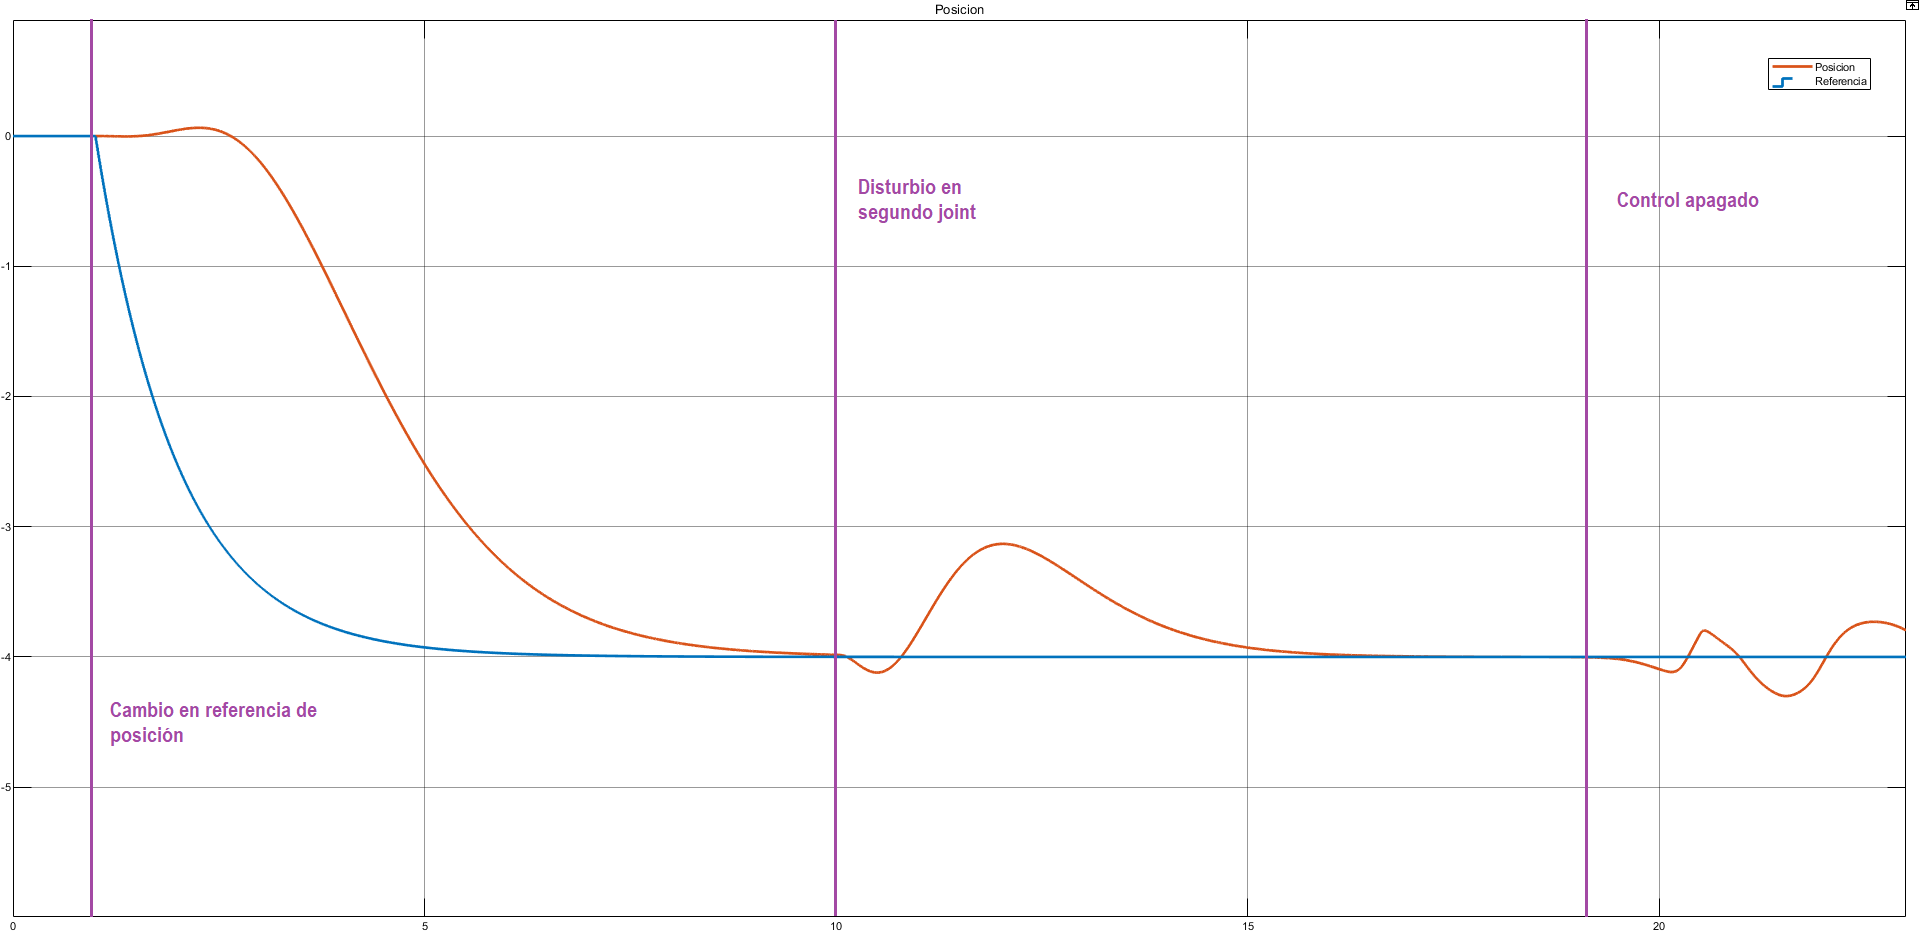
\includegraphics[width=\linewidth]{../Analisis de Resultados/ImagenesAnalisis de Resultados/realim_posref.png}
	\caption{Comparación entre la posición de referencia (azul) y la posición medida (naranja) para el caso de la realimentación ideal de estados.}	
	\label{fig:realim_posref}
\end{figure}

\begin{figure}[H]
	\centering
	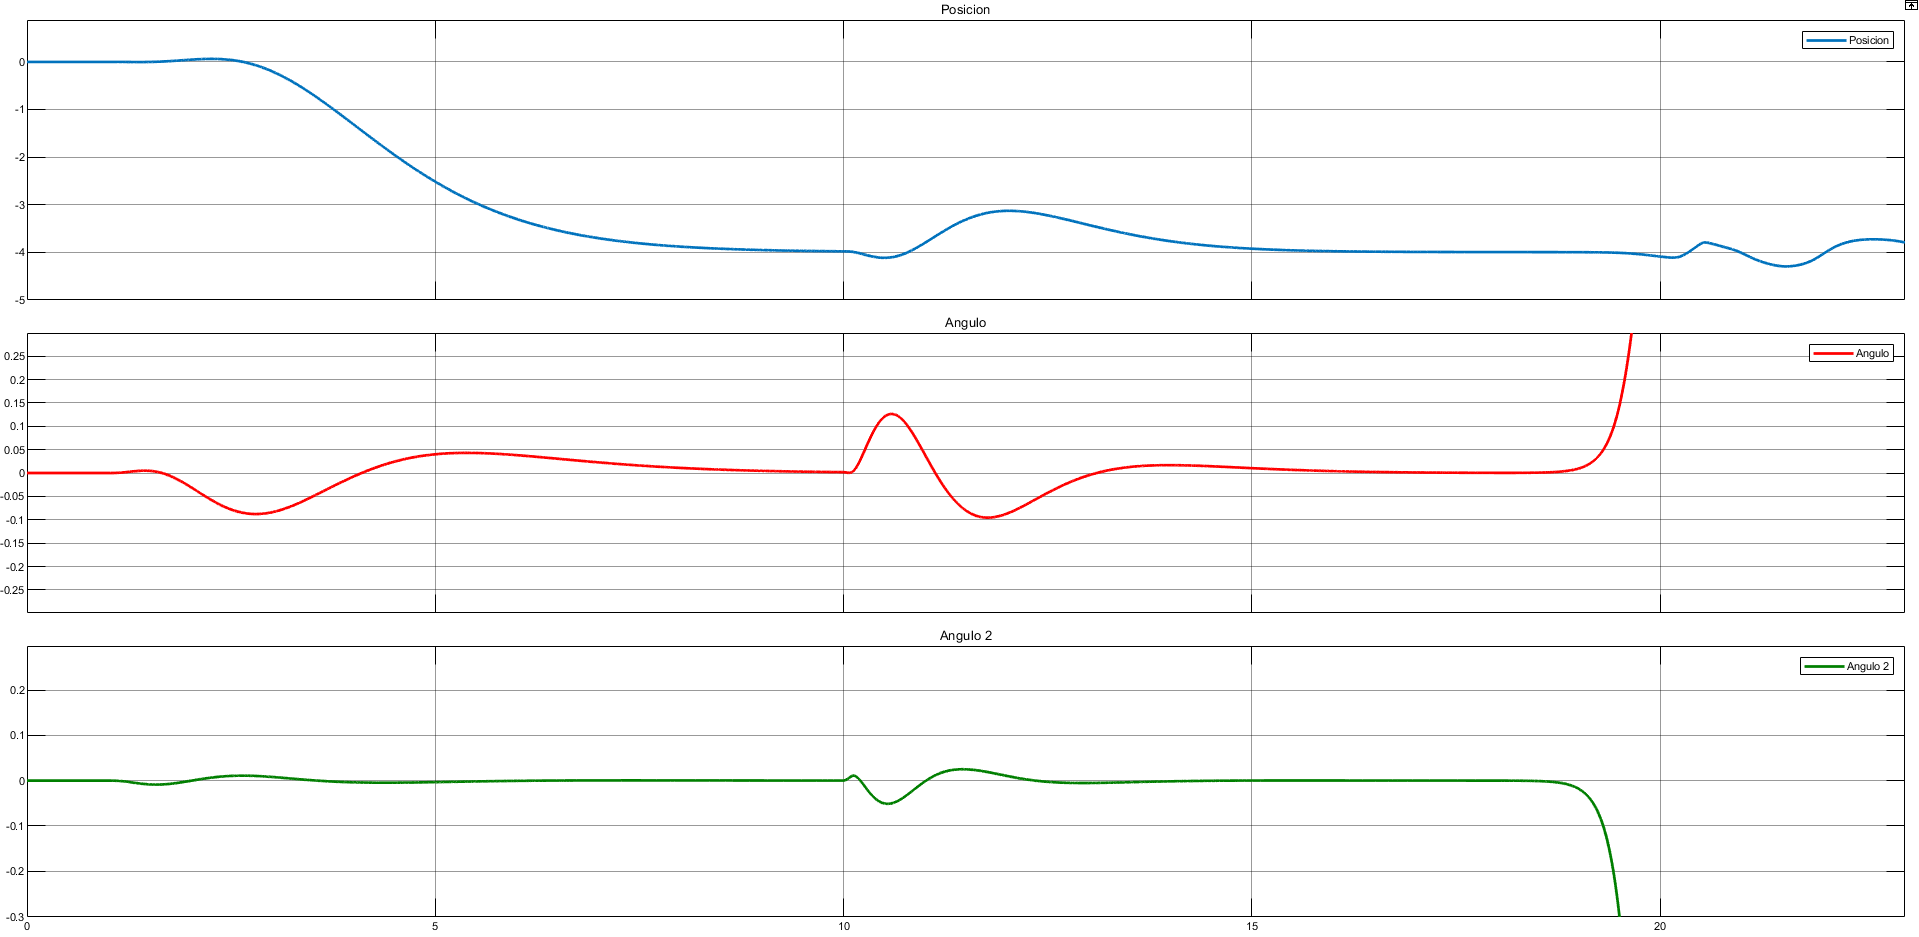
\includegraphics[width=\linewidth]{../Analisis de Resultados/ImagenesAnalisis de Resultados/realim_vars.png}
	\caption{Posiciones angulares y del carrito del sistema para el caso de la realimentación ideal de estados.}	
	\label{fig:realim_vars}
\end{figure}

Para el caso de la realimentación ideal de estados, se puede notar una respuesta al escalón filtrado sin sobrepico para la posición y robustez general ante disturbios. 

\Subsection{Observador}

El sistema con observador presenta mayor sobrepico que el sistema anterior, sin embargo los tiempos para volver a la referencia son similares.

\begin{figure}[H]
	\centering
	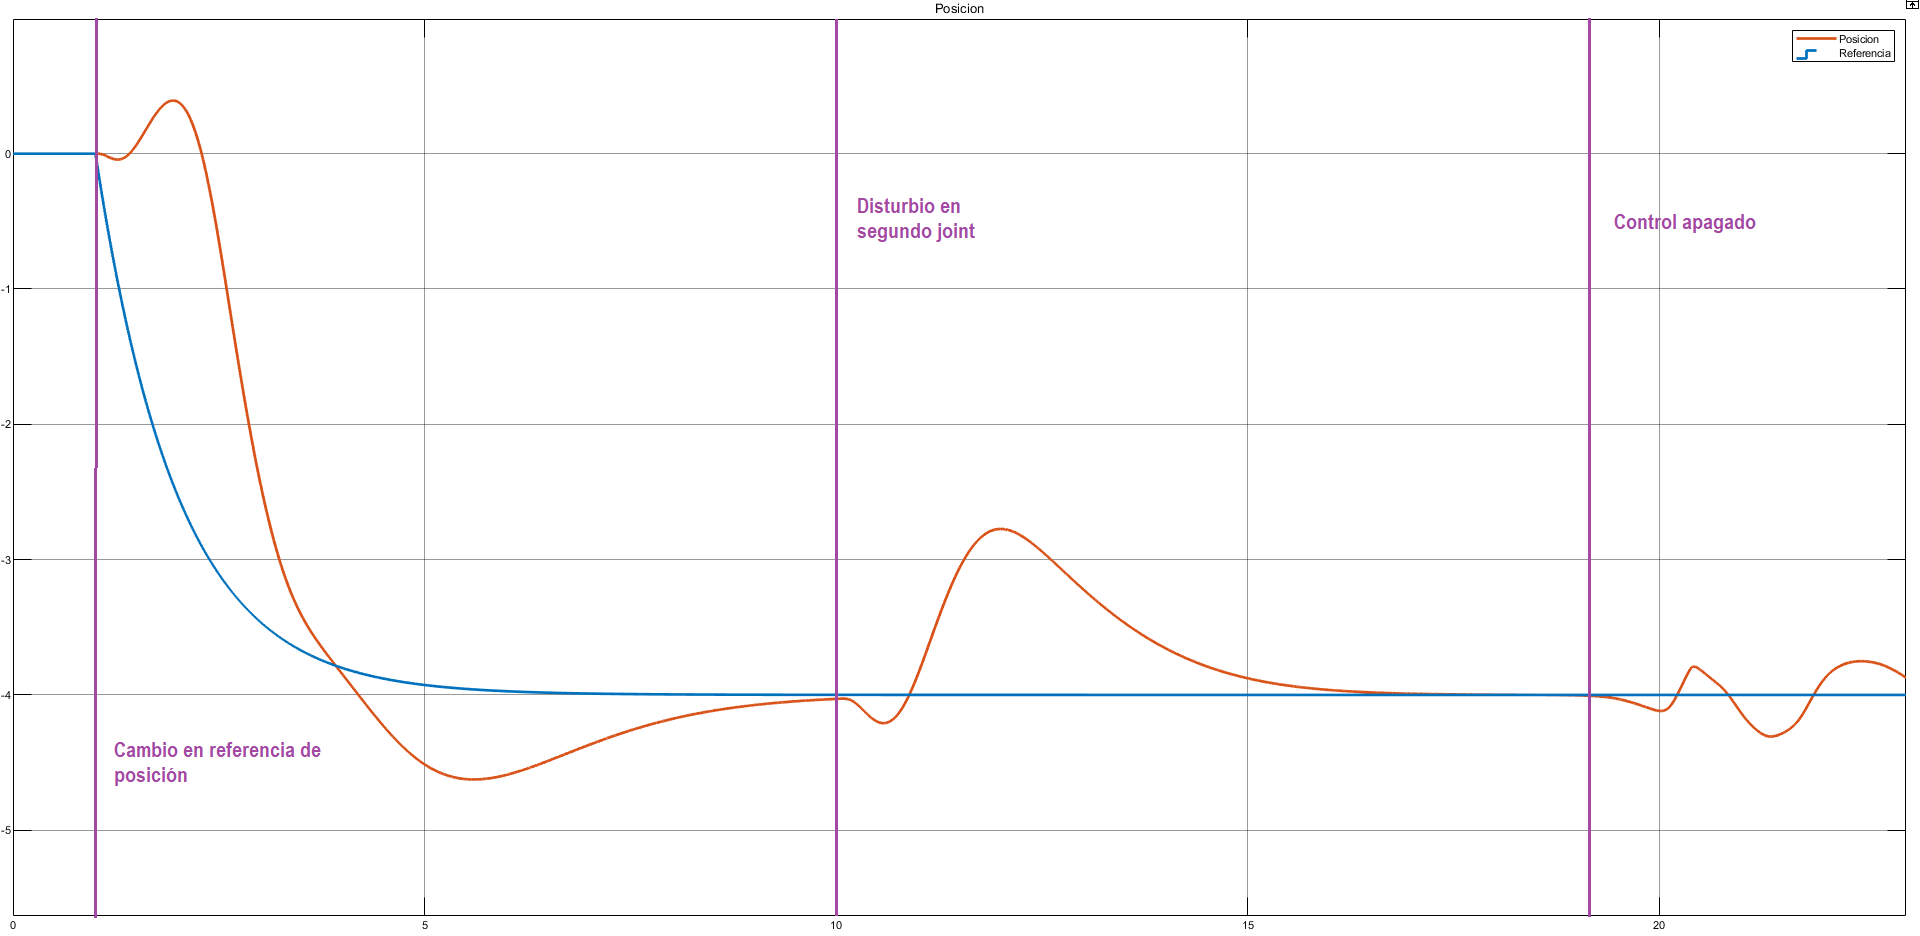
\includegraphics[width=\linewidth]{../Analisis de Resultados/ImagenesAnalisis de Resultados/obsv_posref.png}
	\caption{Comparación entre la posición de referencia (azul) y la posición medida (naranja) para el caso de la realimentación de estados con observador.}	
	\label{fig:obsv_posref}
\end{figure}

\begin{figure}[H]
	\centering
	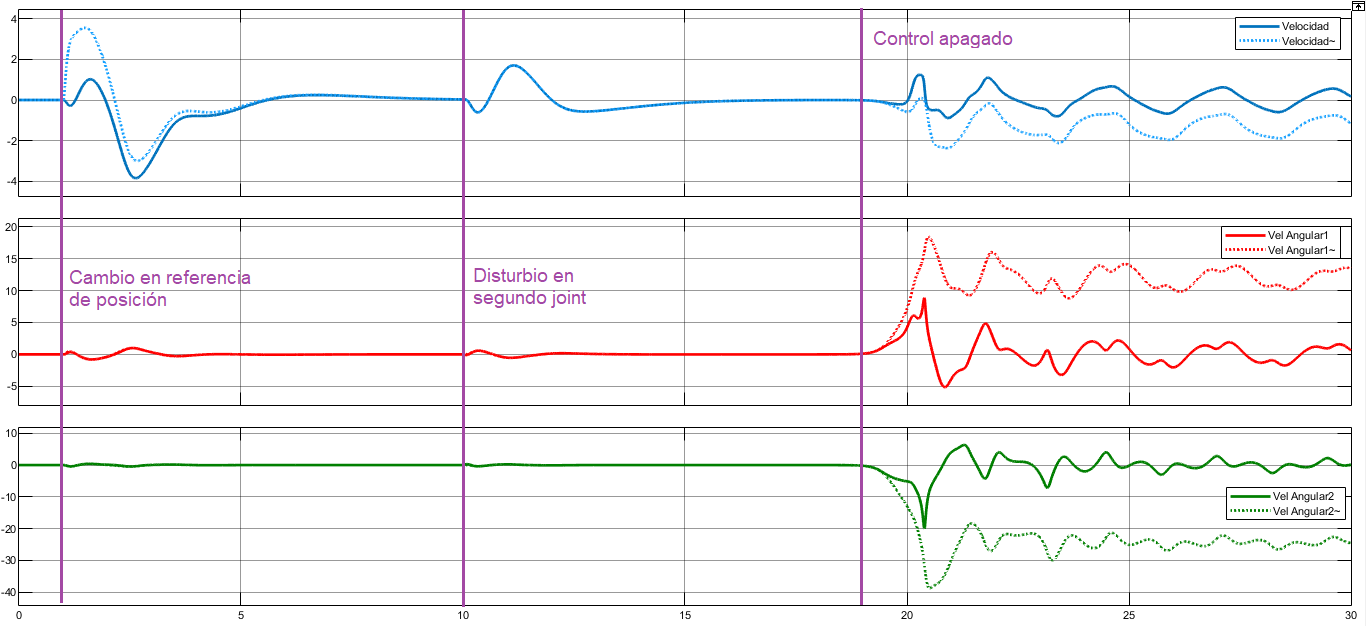
\includegraphics[width=\linewidth]{../Analisis de Resultados/ImagenesAnalisis de Resultados/obsv_vars.png}
	\caption{Posiciones angulares y del carrito del sistema para el caso de la realimentación de estados con observador junto a las estimaciones de las mismas señales del observador en linea punteada.}	
	\label{fig:obsv_vars}
\end{figure}

En la Figura (\ref{fig:obsv_vars}) se puede observar como las señales del observador logran mantenerse muy cerca de las posiciones medidas.

\Subsection{Discretización}

En el caso discreto se debió ralentizar levemente los polos por efecto de la discretización. Esto se puede notar en la Figura (\ref{fig:obsv_disc_posref}) dado que el sistema tarda más en seguir la referencia.

\begin{figure}[H]
	\centering
	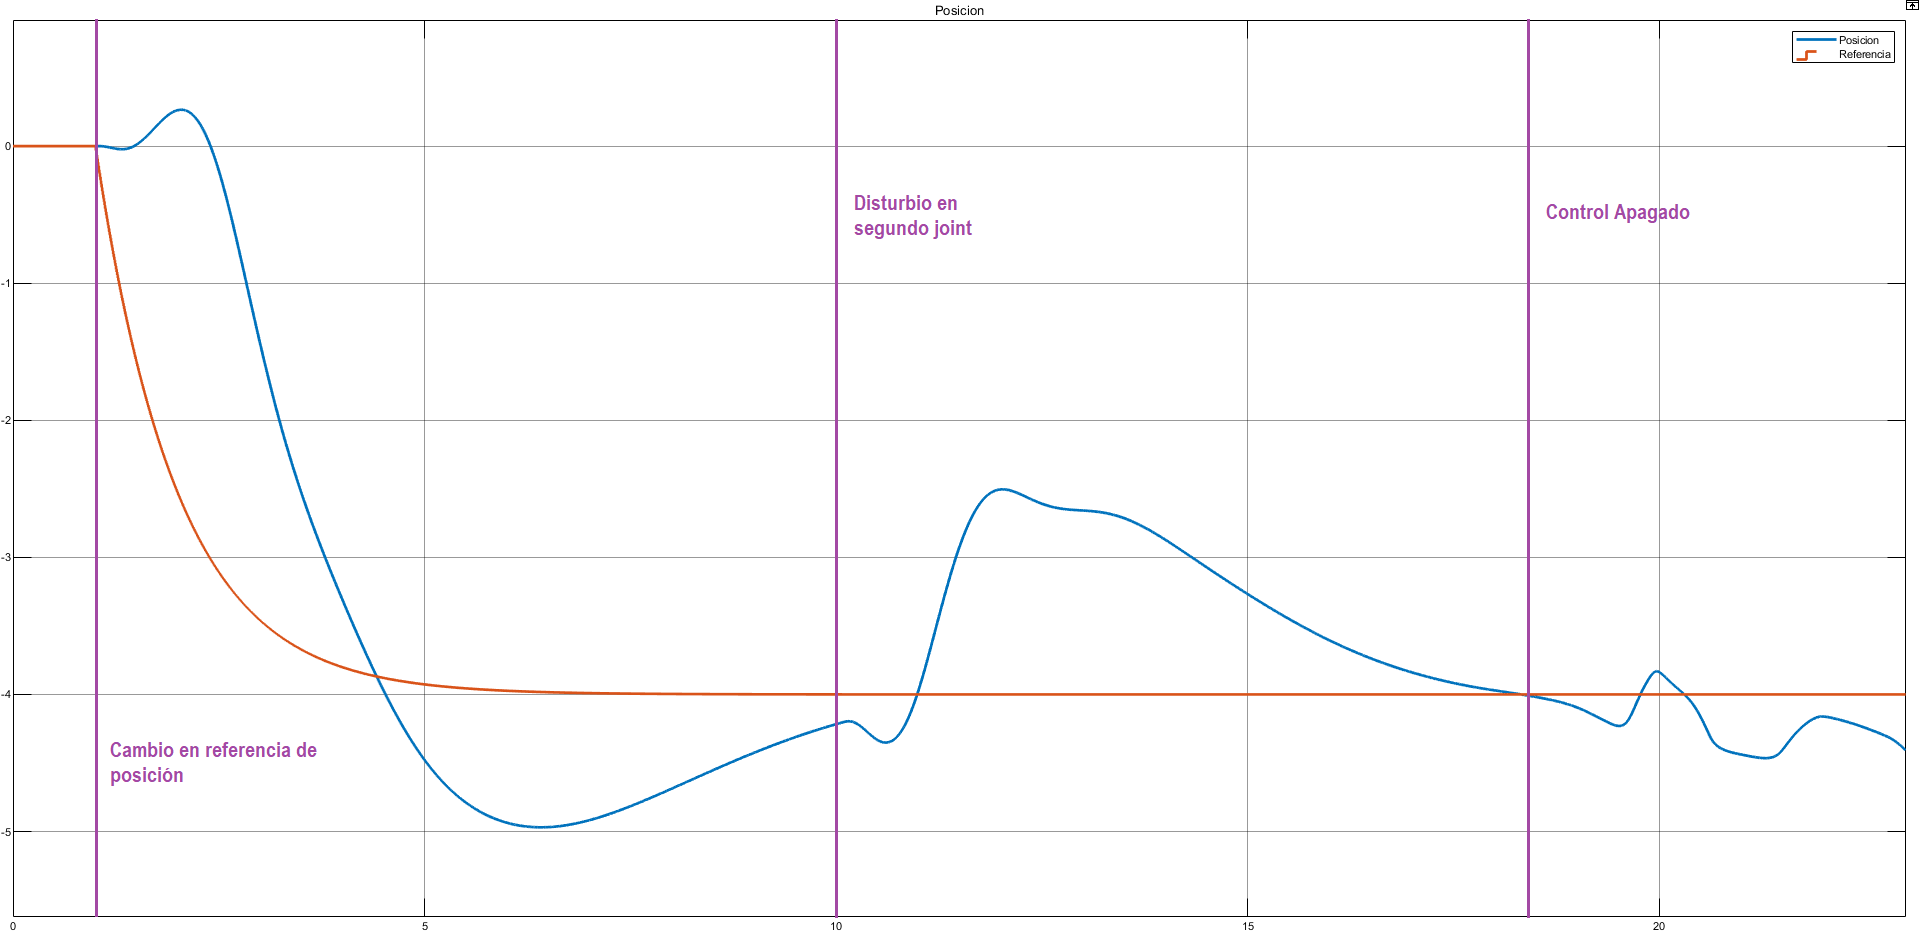
\includegraphics[width=\linewidth]{../Analisis de Resultados/ImagenesAnalisis de Resultados/obsv_disc_posref.png}
	\caption{Comparación entre la posición de referencia (azul) y la posición medida (naranja) para el caso de la realimentación de estados con observador discreto.}	
	\label{fig:obsv_disc_posref}
\end{figure}

En la Figura (\ref{fig:obsv_disc_posdisc}) se puede observar una comparación entre la posición real medida y aquella estimada utilizando el observador discreto. 

\begin{figure}[H]
	\centering
	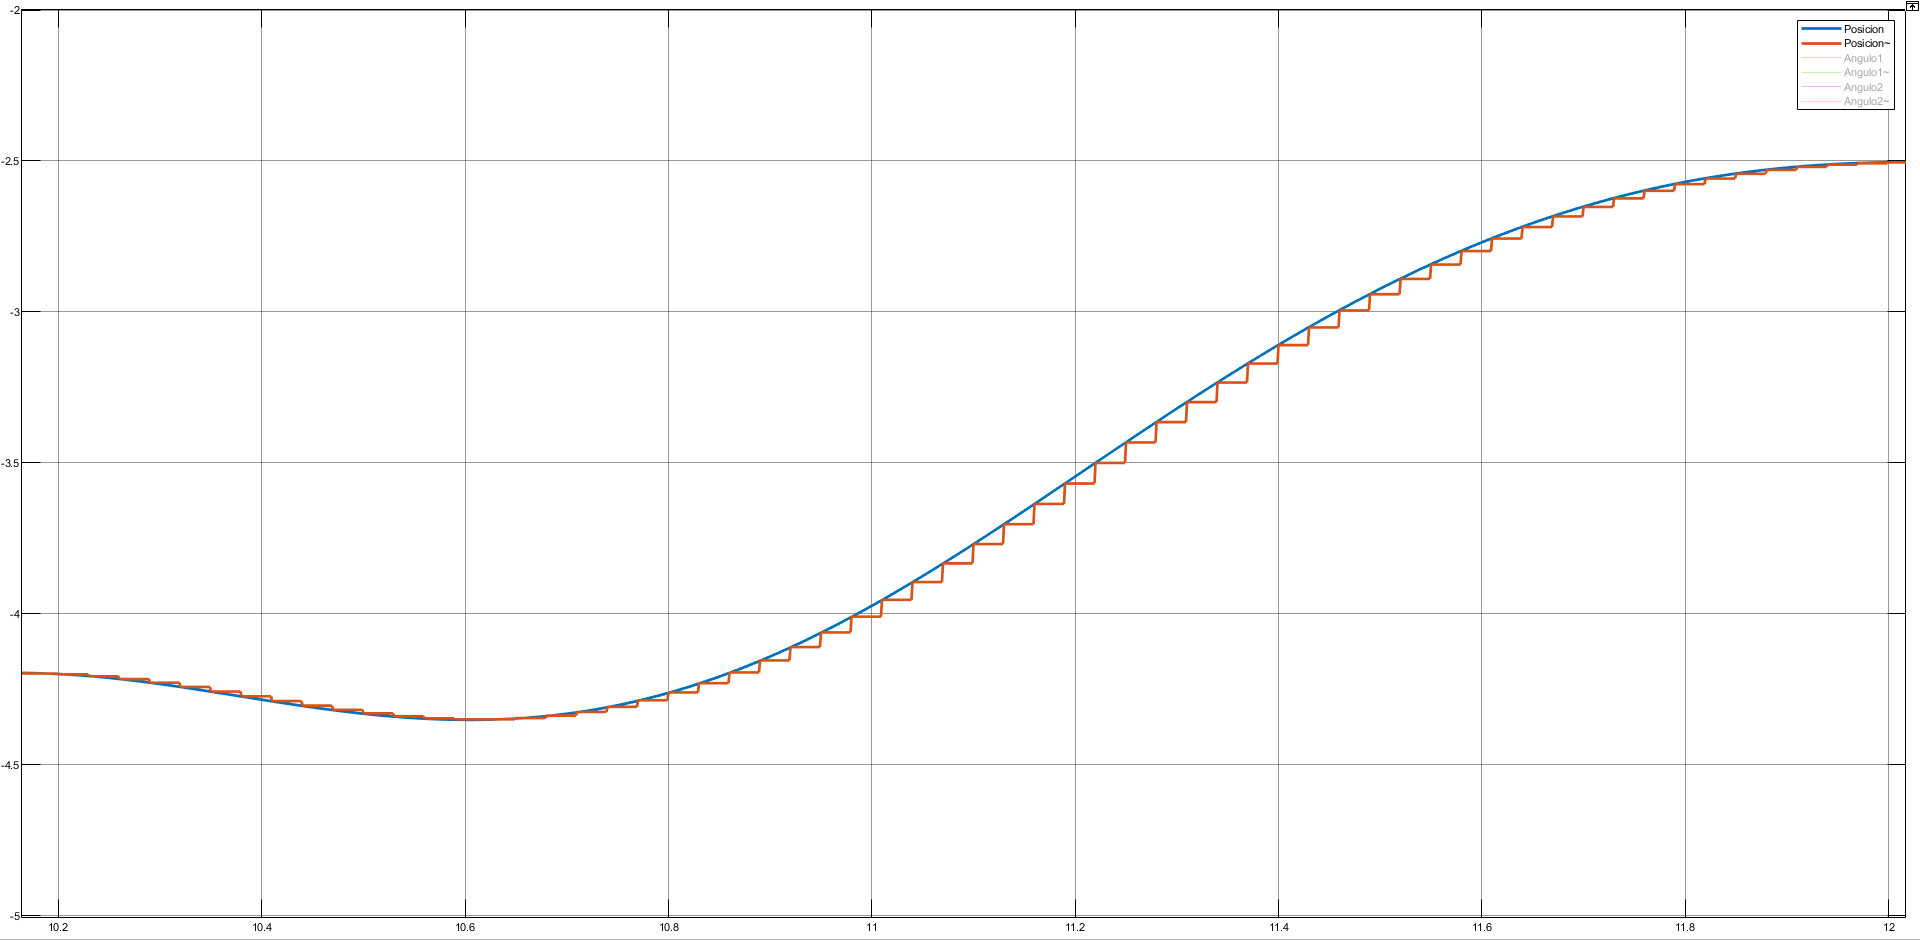
\includegraphics[width=\linewidth]{../Analisis de Resultados/ImagenesAnalisis de Resultados/obsv_disc_posdisc.png}
	\caption{Detalle de las señales de posición real y posición estimada del observador discreto.}	
	\label{fig:obsv_disc_posdisc}
\end{figure}

Finalmente, se pueden observar en la Figura (\ref{fig:disc_vs_ideal_vars}) las posiciones tanto del carrito como las angulares comparadas entre el sistema de realimentación ideal de estados y el sistema con observador discreto. 

Se puede notar cómo debido al muestreo y su introducción del cero en el semiplano derecho el sistema se vuelve mucho más inestable.

\begin{figure}[H]
	\centering
	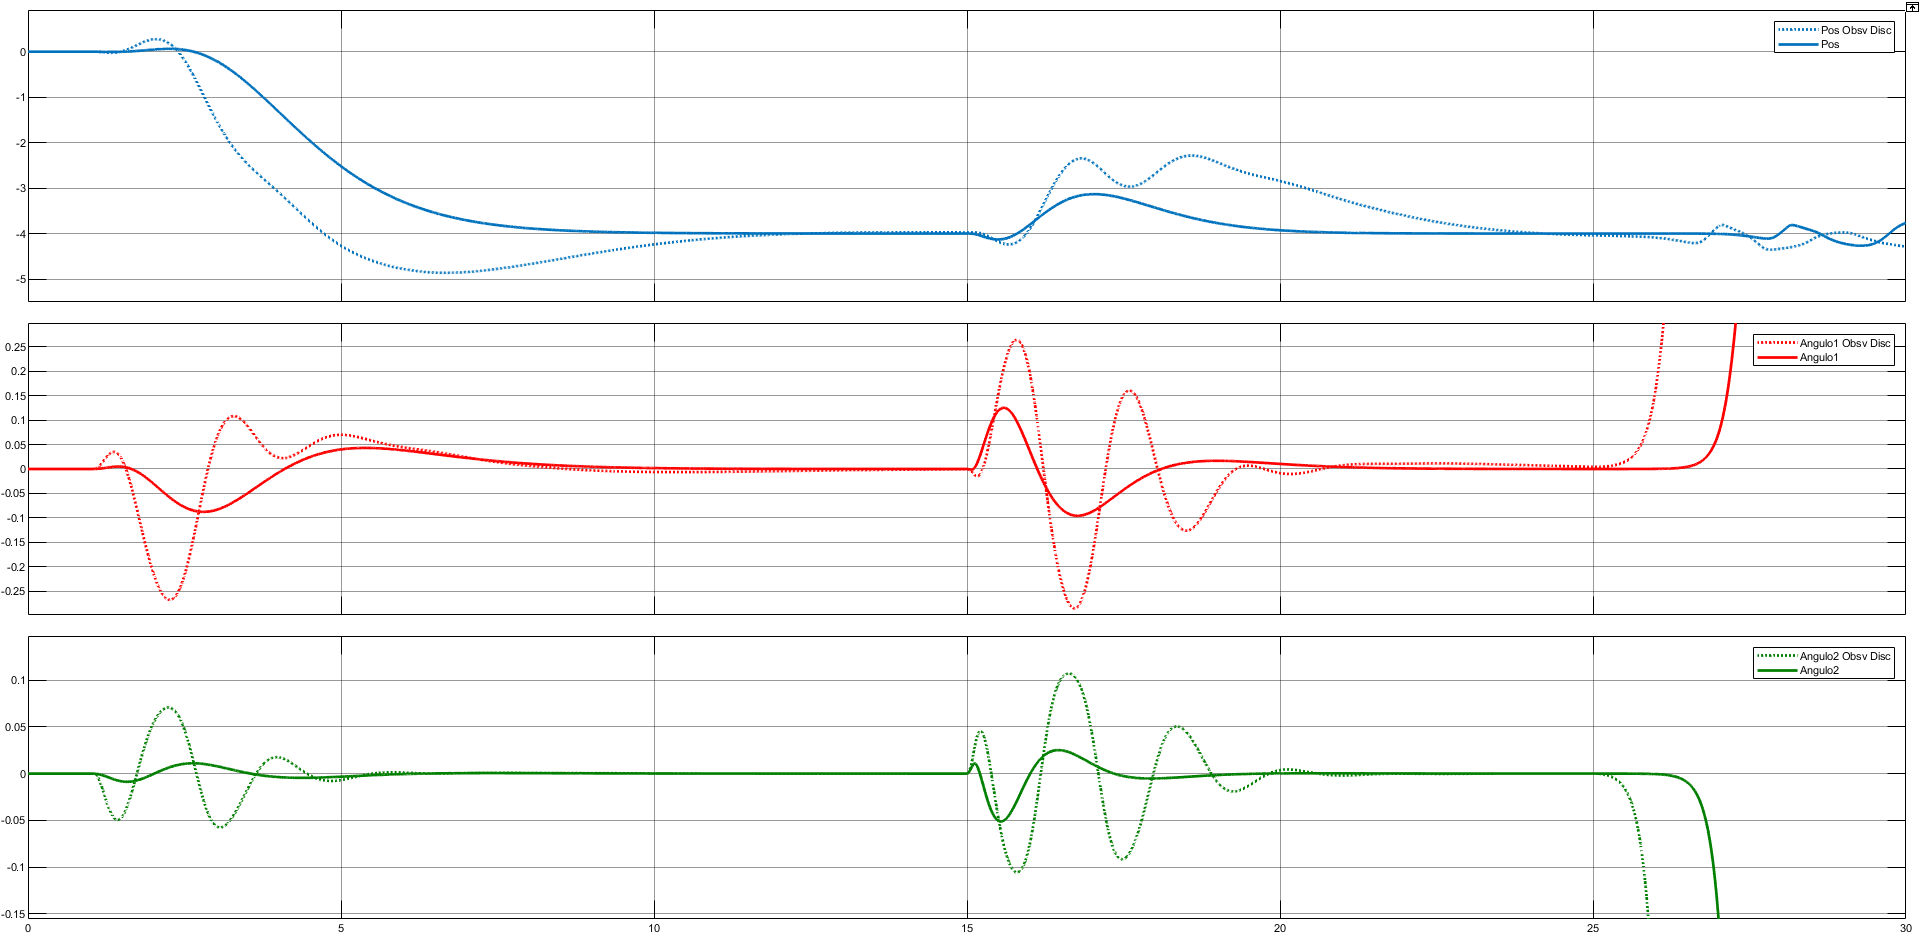
\includegraphics[width=\linewidth]{../Analisis de Resultados/ImagenesAnalisis de Resultados/disc_vs_ideal_vars.png}
	\caption{Comparación de las posiciones angulares y de carrito para los casos de realimentación de estados ideal y realimentación de estados con observador discreto.}	
	\label{fig:disc_vs_ideal_vars}
\end{figure}

PENDIENTE

\Subsection{Integral}
PENDIENTE
\Subsection{Comparativa con péndulo invertido simple}
Para comenzar, la principal diferencia entre estos dos sistemas es la cantidad de variables de estados con los que cuentan ambos sistemas.
Esto se debe a que uno es una versión más compleja mecánicamente del otro.
\begin{figure}[H]
\begin{subfigure}{.5\textwidth}
  \centering
  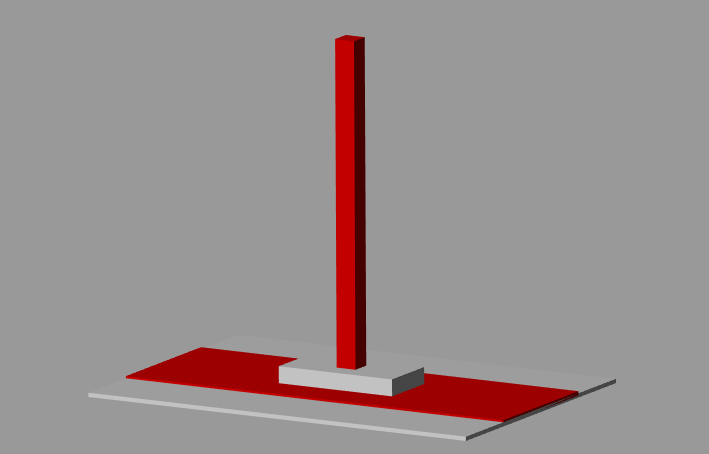
\includegraphics[width=0.95\linewidth]{../Analisis de Resultados/ImagenesAnalisis de Resultados/equilibrio.png}
  \caption{Simple.}
  \label{fig:sfig1}
\end{subfigure}%
\begin{subfigure}{.5\textwidth}
  \centering
  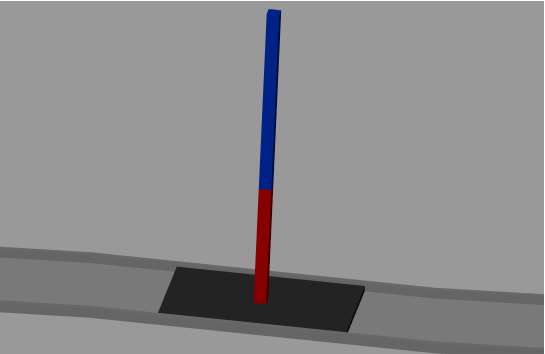
\includegraphics[width=0.95\linewidth]{../Analisis de Resultados/ImagenesAnalisis de Resultados/simscape_double_pendulum.png}
  \caption{Doble.}
  \label{fig:sfig2}
\end{subfigure}
\caption{Péndulo invertido.}
\label{fig:fig}
\end{figure}
Si bien esto es cierto, si se opta por cambiar los parámetros de segundo, haciendo que el segundo link tenga una longitud que tienda a cero, ambos sistemas coinciden, como es de esperarse.

Ambos sistemas son estrictamente observables en todos los casos de fricción tomando mediciones únicamente de la posición por lo explicado anteriormente. Sin embargo, en la realidad, realizar el control del péndulo doble midiendo únicamente la posición resulta mucho mas difícil, que en el caso del péndulo simple.
También resulta curioso que en ambos casos al ampliar el sistema para realizar el control integral con roce y amortiguamiento estos no son controlables.

PENDIENTE
%\end{document}